\documentclass{UoNMCHA}
\usepackage[authoryear]{natbib}
\usepackage{array,booktabs} % For nice tables
\usepackage{amsmath,amsfonts,amssymb} % For nice maths
\usepackage{color}
\usepackage{multicol}
\usepackage{enumerate}
\usepackage{listings}
\usepackage{subfig}
\usepackage{hyperref}
\usepackage[parfill]{parskip}   % For replacing paragraph indenting with a newline instead
\usepackage{tabularx}
\newcolumntype{C}{>{\centering\arraybackslash $}X<{$}}
\usepackage{geometry}
\newif\ifcomment
\commenttrue
\commentfalse
% Number equations per section
\numberwithin{equation}{section}

\hypersetup{
%    bookmarks=true,         % show bookmarks bar?
%    unicode=false,          % non-Latin characters in AcrobatÕs bookmarks
%    pdftoolbar=true,        % show AcrobatÕs toolbar?
%    pdfmenubar=true,        % show AcrobatÕs menu?
%    pdffitwindow=false,     % window fit to page when opened
%    pdfstartview={FitH},    % fits the width of the page to the window
%    pdftitle={My title},    % title
%    pdfauthor={Author},     % author
%    pdfsubject={Subject},   % subject of the document
%    pdfcreator={Creator},   % creator of the document
%    pdfproducer={Producer}, % producer of the document
%    pdfkeywords={keyword1} {key2} {key3}, % list of keywords
%    pdfnewwindow=true,      % links in new window
    colorlinks=true,       % false: boxed links; true: colored links
    linkcolor=blue,          % color of internal links
    citecolor=blue,        % color of links to bibliography
%    filecolor=magenta,      % color of file links
    urlcolor=blue           % color of external links
}

\definecolor{light-gray}{gray}{0.95}
\definecolor{myblue}{RGB}{20,105,176}
\definecolor{myorange}{RGB}{255,140,0}
\definecolor{mygrey}{RGB}{64,64,64}
\definecolor{MATLABKeyword}{rgb}{0,0,1}
\definecolor{MATLABComment}{rgb}{0.1328125,0.54296875,0.1328125}
\definecolor{MATLABString}{rgb}{0.625,0.125,0.9375}

\lstset{language=Matlab,
    basicstyle=\small\ttfamily,
    keywordstyle=\color{MATLABKeyword},
    %identifierstyle=,
    commentstyle=\color{MATLABComment},
    stringstyle=\color{MATLABString},
    numberstyle=\tiny,
    %numbers=left,
    basewidth=0.5em}
\lstset{
language=C,
numbers=none,
xleftmargin=1cm,
frame=tblr,
classoffset=0,
morekeywords={LED_BUILTIN,HIGH,LOW,OUTPUT,INPUT,INPUT_PULLUP},keywordstyle=\color{myblue},
classoffset=1,
morekeywords={analogWrite,pinMode,write,Serial,begin,print,println,digitalWrite,delay,Stepper,step,setSpeed},	keywordstyle=\color{myorange},
classoffset=0,
commentstyle=\color{mygrey},
breaklines=true,
postbreak=\space //...
}

\firstpage{1}    % Set page number for first page
\UoNMCHAreportNo{ELEC1710   } %Report number
\UoNMCHAyear{ }   % Year
\shorttitle{ELEC1710 - Lab 3} %For odd pages
%%%%%%%%%%%%%%%%%%%%%%%%%%%%%%%%%%%%%%%%%%%%%%%%%%%%
\begin{document}
\title{Lab 3:\\Breadboard Implementation of a Combinational Logic Circuit \\ \ \\
{\small ELEC1710    \\ 
}}
%\author[UoNMCHA]{Student Name}
%\address[UoNMCHA]{
%Student of Mechatronics Engineering,\\
%The University of Newcastle, Callaghan, NSW 2308, AUSTRALIA \\
%Student Number: 3...... \\
%E-mail: \href{mailto:First.Last@uon.edu.au}{\textsf{First.Last@uon.edu.au}}}
%%%%%%%%%%%%%%%%%%%%%%%%%%%%%%%%%%%
\maketitle
\onecolumn

\vspace{-5mm}

\section{Introduction}

In this lab you will be given a Boolean expression and are required to implement that expression on a breadboard using a combination of AND, OR and NOT gates. This lab will prepare you for Part B of your project.

\section{Equipment}

To perform this lab you will require:

\begin{itemize}
    \item A breadboard and associated power supply
    \item 2x Tactile push button switches
    \item 2x 1k~$\Omega$ resistors
    \item 2x 10k~$\Omega$ resistors. (1K will also work if 10K not available)
    \item 1x Quad 2-input AND gate chip
    \item 1x Quad 2-input OR gate chip
    \item 2x LEDs
\end{itemize}

\section{Reference Data}

There are many different chips available which implement the AND, OR and NOT operations. These are typically based off either the 74- series (TTL) or 4000 series (CMOS) chips.

From the 74- Series you could use the following:

\begin{itemize}
    \item 7408 Quad 2-input AND
    \item 7432 Quad 2-input OR
\end{itemize}

The same functions are implemented in the following 4000 series CMOS devices:

\begin{itemize}
    \item 4071 Quad 2-input OR
    \item 4081 Quad 2-input AND
\end{itemize}

Note that the numbers printed on chips will typically include a \textit{logic family} code. For example:

\begin{itemize}
    \item 74HCxx - High speed CMOS
    \item 74LSxx - Low power schottky
\end{itemize}

Devices from different logic families differ in speed, power consumption, etc while maintaining the same pin configuration.

\subsection{Pinouts}

 Refer to Figures \ref{NOTPinout}, \ref{ANDPinout} \& \ref{ORPinout} for pinouts of the NOT, AND \& OR gates, respectively. Note that the pinouts differ between some 74xx and 4xxx series devices.

\begin{figure}[h!]
\centering
    \subfloat[4081 Pinout]{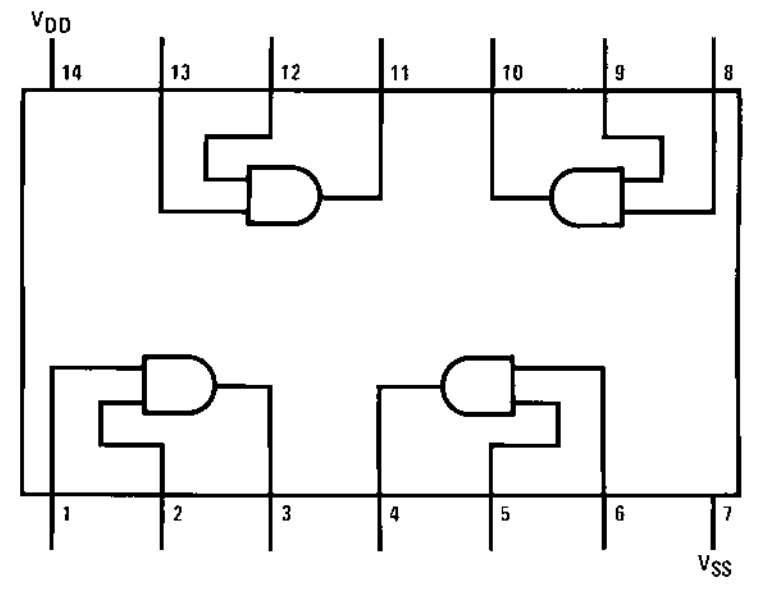
\includegraphics[width=0.4\textwidth]{Figures/4081}}
    \qquad
    \subfloat[7408 Pinout]{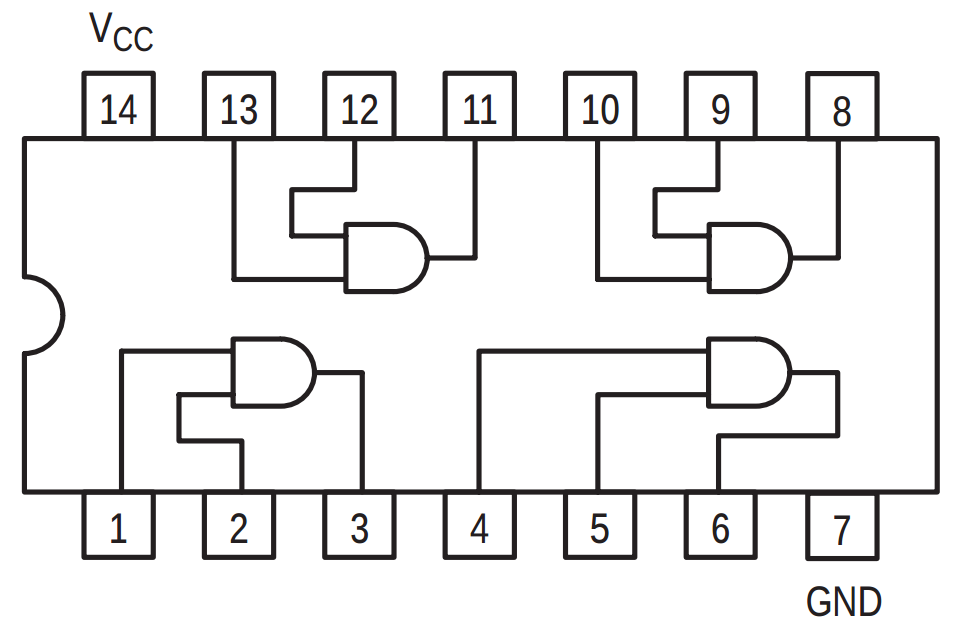
\includegraphics[width=0.4\textwidth]{Figures/7408}}
    \caption{Quad 2-input AND gate pinouts. Note that $V_{DD}$ is another name for $V_{CC}$.}
    \label{ANDPinout}
\end{figure}

\begin{figure}[h!]
\centering
    \subfloat[4071 Pinout]{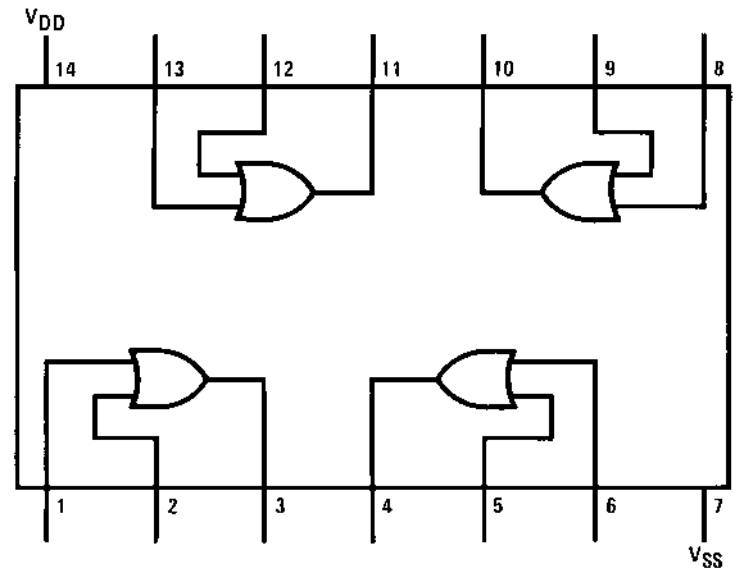
\includegraphics[width=0.4\textwidth]{Figures/4071}}
    \qquad
    \subfloat[7432 Pinout]{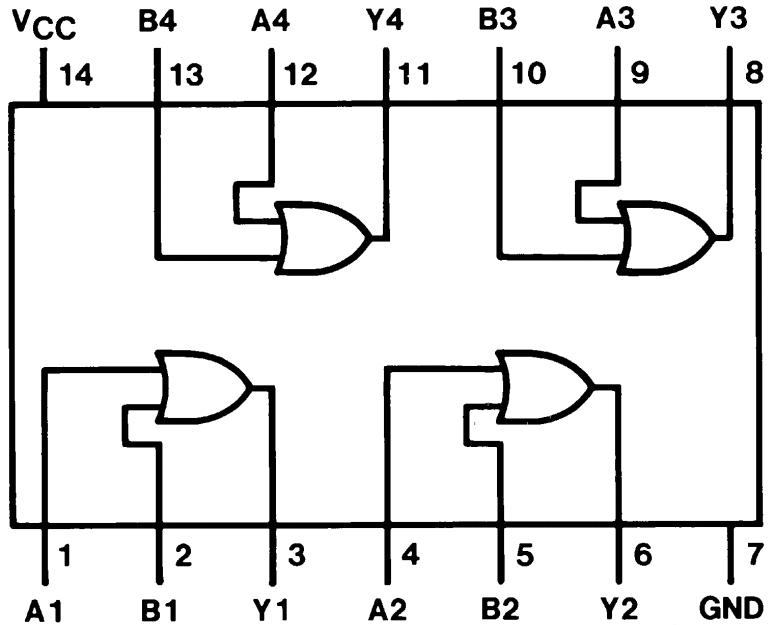
\includegraphics[width=0.4\textwidth]{Figures/7432}}
    \caption{Quad 2-input OR gate pinouts. Note that $V_{DD}$ is another name for $V_{CC}$.}
    \label{ORPinout}
\end{figure}

\begin{figure}[h!]
\makebox[\textwidth][c]{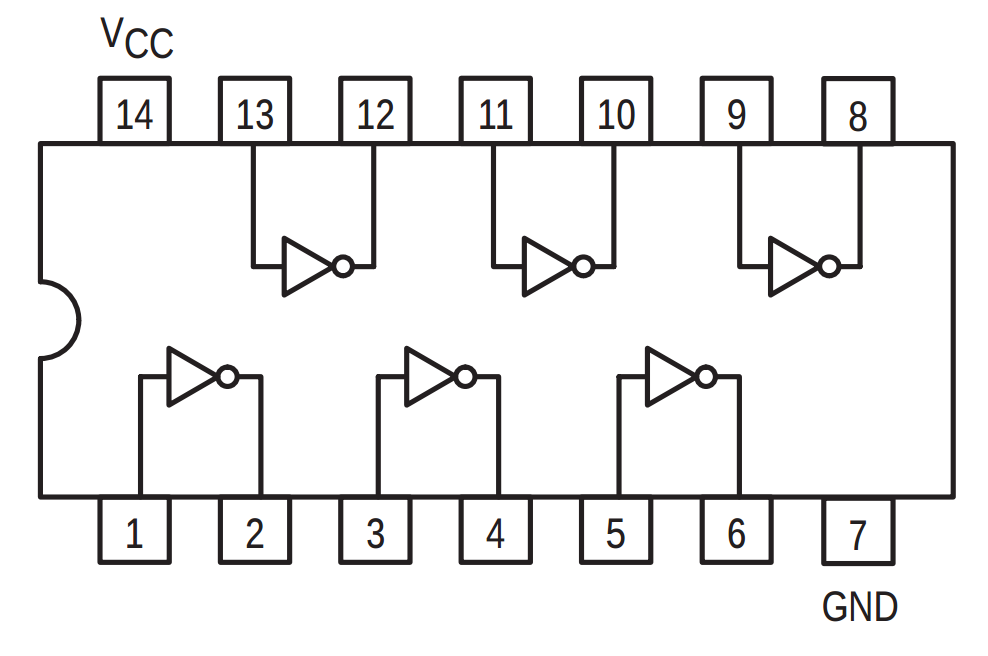
\includegraphics[width=0.4\textwidth]{Figures/7404}}
\caption{Pinout for 7404 and 4069 hex inverter chips.}
\label{NOTPinout}
\end{figure}

\section{Prework}

Your lab task is to implement the following Boolean expressions:

\begin{equation} \label{eq:sum}
S = A \overline{B} + \overline{A} B
\end{equation}
\begin{equation} \label{eq:carry}
C = AB    
\end{equation}


These expressions implement a binary half-adder where $S$ and $C$ correspond to the \textit{sum} and \textit{carry} outputs (respectively) and will be connected to LEDs. The variables $A$ and $B$ are the two binary bits to be added and will be generated by the push buttons with pull down resistors as in previous labs.

\textbf{Tasks:}
\begin{enumerate}
    \item Complete the truth table for Equations \ref{eq:sum} and \ref{eq:carry}:

    \begin{tabularx}{0.4\textwidth}{@{\rule[-3ex]{0pt}{7ex}}|*{7}{C|}}
    \hline
    A & B & S & C \\
    \hline
    & & & \\
    \hline
    & & & \\
    \hline
    & & & \\
    \hline
    & & & \\
    \hline
    \end{tabularx}
    
    \item Draw a logic circuit implementation of Equations \ref{eq:sum} and \ref{eq:carry} on the next page. Include the switches, their pull down resistors and output LEDs with their resistors. Use 10k$\Omega$ resistors for the switches and 1k$\Omega$ resistors for the LEDs.
    \item Annotate the circuit with chip pin numbers around each gate. Use either the 7400 series or 4000 series pinout depending on what is available in the lab.
\end{enumerate}
\vspace{5cm}
\pagebreak
Draw the circuit diagram on this page
\pagebreak

\section{Construction Procedure}
%You have been provided with two breadboards so that the 7-segment display built in the previous lab can be used as a display module in later labs. Build %this circuit on the unused breadboard.
\begin{enumerate}
    \item Insert the power supply unit onto the breadboard and confirm that the output voltages are set to +3.3~V as done in previous labs.
    \item Insert two tactile switches and wire them up in an \textit{active high} configuration as done in previous labs.
    \item Insert the three logic chips into the breadboard leaving a 1~cm gap between them so they can be easily removed.
    \item Connect all three $V_{cc}$ pins to +3.3~V.
    \item Connect all three GND pins to breadboard ground.
    \item Insert the two LEDs close to where they will be connected to their logic chips. Bend their legs so that the negative (cathode, short leg) is inserted directly into breadboard ground and the other leg is in the main breadboard work area. Make sure they don't connect directly to any chip pins.
    \item Use 1k$\Omega$ resistors to connect the LED's positive terminal to the correct logic chip pin.
    \item Following your schematic make all other connections as required. Be systematic, cross off connections as you make them.
    \item Power on the circuit and confirm that its output matches your truth table. If it does not work correctly you can use the Saleae analyser to help debug your circuit by connecting probes to the inputs, outputs, and any intermediate signals.
\end{enumerate}

\end{document}